\section{Figures}\label{sec:figuras}
\blindtext. Figure \ref{fig:imagen 1}

\begin{figure}[h]
    \centering
    
\includegraphics[width=0.8 \textwidth]{image.jpg}
    \caption{Descripcion de la imgen}
    \label{fig:imagen 1}
\end{figure}

\blindtext. Figure \ref{fig:imagen 2}

\begin{figure}[H]
    \centering
    \subfloat[Descripcion grafica 1 \label{subfig:grafica11}]{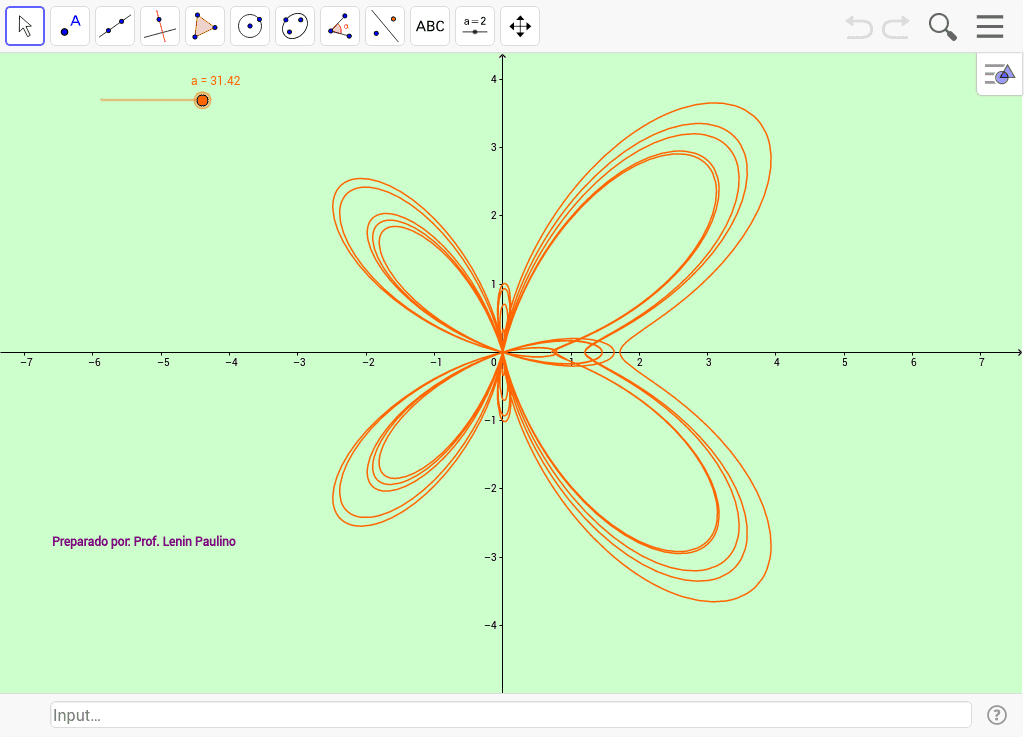
\includegraphics[width=0.4 \textwidth,valign=c]{grafica1.png}}
    \hfill
    \subfloat[Descripcion grafica 2 \label{subfig:grafica12}]{
\includegraphics[width=0.4 \textwidth,valign=c]{grafica2.png}}

    \caption{Descripcion de la imagen 2}
    \label{fig:imagen 2}
\end{figure}